%!TEX root=thesis.tex
\chapter{Background}

\section{Motivation}

Some physicists believe that quantum physics is on the cusp of a ``second quantum revolution''.\cite{quantum-rev} The ability to probe quantum systems with finer precision and control them to a greater extent, as opposed to passively observing emergent phenomena that arise, has potential to radically transform many different areas, from sensing to simulation quantum computing.

Two specific examples where quantum control can be readily applied include NMR spectroscopy and bath engineering. In NMR spectroscopy, the collective magnetization of spin-1/2 protons in a sample can be measured, and the resulting signal informs the particular chemical environments the spins are in. However, for solid-state samples, magnetic dipolar interactions between spins lead to state decoherence
% TODO is ^ correct?
and overwhelm the signal and inhibit our ability to learn about the chemical environments. However, various methods have been developed to effectively \emph{decouple} the magnetic dipolar interactions between spins, improving the signal drastically.

Magnetic dipole interactions between a central spin and many surrounding bath spins (such as an NV center surrounded by many P1 centers) also leads to unwanted effects, in this case a decay of the central spin coherence time. Long coherence times for the system of interest are desirable, and finding ways to decouple interactions between the central spin and bath spins would help that endeavor.

\section{Important Quantum Mechanics Concepts}

This section is meant to present some fundamental ideas that will be used throughout, but for a more thorough description of quantum mechanics see
\cite{mcintyre2012quantum, sakurai2017modern}.
.
In all equations that follow, $\hbar = 1$ is assumed.

% state of system <-> density operator
Given a quantum system, a general state can be represented by a density operator $\rho(t)$. The density operator encapsulates all known information about the quantum system, specifically the expectation values associated with well-defined observable. For an observable $A$, the expectation is given by
\begin{equation}\label{eq:measure}
    \langle A \rangle = \Tr{\rho A}
\end{equation}

The time evolution of the density operator is given by
\begin{equation}\label{eq:density-time}
    \rho(t) = U(t) \rho(0) U(t)^\dagger
\end{equation}
where the unitary operator $U$ is the ``propagator'' defined by
\begin{equation}\label{eq:propagator-de}
    i \ddt{U(t)} = H(t) U(t), U(0) = \identity
\end{equation}
% The two equations above can be combined to yield the Liouville-Von Neumann equation, which explicitly shows the density operator's time evolution from the system Hamiltonian.
% \begin{equation}
%     i \ddt{\rho(t)} = [H(t), \rho(t)]
% \end{equation}

When the Hamiltonian is time-independent or if the Hamiltonian commutes with itself at different points in time (i.e. $[H(t_1), H(t_2)] = 0$), equation~\ref{eq:propagator-de} can be solved to obtain the propagator
\begin{equation}\label{eq:propagator-ti}
    U(t) = \text{exp}\left[ {-i \int_0^t H(t') dt'} \right]
\end{equation}
However, if the Hamiltonian is time-dependent and doesn't commute with itself at different times, then the above equation is not valid. This difficulty with time-dependent Hamiltonians and methods with dealing with them are further discussed in~\ref{sec:AHT}.

In many cases it can be helpful to consider the \emph{interaction frame} of a particular interaction. If the Hamiltonian is expressed as the sum of two terms
\[
H(t) = H_A(t) + H_B(t)
\]
then there is a unitary operator $U_A(t)$ given by
\begin{equation}\label{eq:interaction-propagator}
    \frac{d}{dt} U_A(t) = -i H_A(t) U_A(t), \, U_A(0) = \identity
\end{equation}
that maps from the interaction frame to the lab frame.
The dynamics in the interaction frame are described by the interaction frame Hamiltonian $\widetilde{H}(t) = {U_A(t)}^{\dagger} H_B(t)U_A(t)$
\[
\frac{d}{dt}\widetilde{U}(t) = -i \widetilde{H}(t)\widetilde{U}(t),\, \widetilde{U}(0) = \identity
\]
The propagator in the lab frame $U(t)$ is related to $\widetilde{U}(t)$ by first time evolution in the interaction frame, then mapping from the interaction frame to the lab frame
\[
U(t) = U_A(t)\widetilde{U}(t).
\]

\section{Spin-1/2 Systems and Nuclear Magnetic Resonance}

A spin-1/2 particle (such as an electron or proton) has two possible values for its intrinsic angular momentum or ``spin,'' so the corresponding Hilbert Space for a single spin-1/2 particle has dimension two. $I_x, I_y$ and $I_z$ denote the operators for nuclear spin along $x, y$, and $z$, respectively. For a collection of $N$ spin-1/2 particles, the corresponding Hilbert Space has dimension $2^N$.
For an ensemble of spins, the term $I_z^{(j)}$ is shorthand for a tensor product of operators, all identity except for the $j$th operator
\[
I_z^{(j)} = \identity \otimes \identity \otimes \dots \otimes I_z \otimes \dots \otimes \identity
\]
Similarly, the term $I_z^{(j)}I_z^{(k)}$ is shorthand for a product of identity operators except for the $j$th and $k$th operators.

Nuclear magnetic resonance (NMR) encompasses the study of nuclear spins and the various interactions they have with external fields and with each other.
The key interactions considered in this work are given below, but a complete description of the interactions present in NMR can be found in \cite{1976ii}.%
\footnote{The quadrupolar interaction and J coupling are not considered here, but it's good to remember they're still there in general.}
\begin{align}\label{eq:nmr-ham}
    H(t) &= H_Z + H_\text{CS} + H_D + H_\text{rf}(t) \\
    H_Z &= \omega_0 \sum_j I_z^{(j)} \\
    H_\text{CS} &= \sum_j \delta_i I_z^{(j)} \\
    H_D &= \sum_{j,k} d_{jk} \left( 3I_z^{(j)}I_z^{(k)} - \mathbf{I^{(j)}} \cdot \mathbf{I^{(k)}} \right) \\
    \label{eq:nmr-ham-rf}
    H_{\text{rf}}(t) &=  u_1(t) \omega_1 \sum_j I_x^{(j)}
\end{align}
The Zeeman interaction $H_Z$ captures the coupling of spins to the main external magnetic field along the z-axis. The oscillation frequency associated with the Zeeman interaction is called the Larmor frequency $\omega_0 = \gamma_i B_0$, and only differs between spins if the gyromagnetic ratio differs (e.g. between $H^1$ and $C^{13}$). We assume going forward that all spins are of the same species.%
\footnote{The external magnetic field $B_0$ also varies from spin to spin due to experimental imperfections, but those field inhomogeneities are also ignored.}
The chemical shift interaction $H_{\text{CS}}$ captures the local magnetic field differences for each spin, and the dipolar interaction between spins is represented by $H_D$. Finally, $H_\text{rf}(t)$ is the interaction between the spins and a time-varying transverse magnetic field along the x-axis.%
\footnote{The reason it is labeled as $H_\text{rf}$ is because the field's oscillation frequency is matched to the Larmor frequency $\omega_0$ which is in the radiofrequency range.}
The time-independent terms in the Hamiltonian ($H_Z + H_{\text{CS}} + H_D$) are referred to as the internal Hamiltonian or $H_{\text{int}}$.

% % TODO include this if I have time?
% \begin{figure}[H]
%     \centering
%     \includegraphics[width=.5\textwidth]{example-image}
%     \caption{NMR experimental setup.}
%     \label{fig:NMR-setup}
% \end{figure}

In an NMR spectrometer, a sample is placed into an external magnetic field $B_0$ (defining the principal axis or z-axis).
% TODO elaborate on this if I need to, otherwise cut...
% The spins in the sample reach thermal equilibrium and are characterized by the density operator
% \[
% \rho_{\text{eq}} = \frac{
%     e^{-\beta H_{\text{int}}}
%     }{
%     \Tr{
%         e^{-\beta H_{\text{int}}}
%      }
%     }
% \]
% The dominant term in the internal Hamiltonian is $H_Z$, so the first-order approximation for $\rho_{\text{eq}}$ is given by
% \[
% \rho_{\text{eq}} \approx \identity + \epsilon \sum_j I_z^{(j)}
% \]
% The identity term does not contribute to the system's dynamics ($U \identity U^\dagger = \identity$) so we can focus on the collective spin term $\sum_j I_z^{(j)}$.
If we only consider the Zeeman term $H_Z$, then the propagator $U_Z(t)$ is given by
\[
U(t) = \exp \left( -i \omega_0 t \sum_j I_z^{(j)} \right)
\]
which corresponds to rotation about the z-axis with angular velocity $\omega_0$. An intuitive understanding is that the spins collectively precess about the magnetic field. The interaction frame of the Zeeman term, also known as the ``rotating frame,'' is a helpful frame to work in for many cases. The interaction propagator (equation~\ref{eq:interaction-propagator}) is given by $U_Z(t)$ above, and so the interaction frame Hamiltonian is
\begin{align*}
    \widetilde{H}(t) &= {U_Z(t)}^{\dagger} \left[ H_\text{CS} + H_D + H_\text{rf}(t) \right] U_Z(t) \\
        &= H_\text{CS} + H_D + \widetilde{H_\text{rf}}(t)
\end{align*}
Both $H_\text{CS}$ and $H_D$ commute with $H_Z$ and therefore commute with $U_Z(t)$. The rf field $H_\text{rf}(t)$ does not commute with $H_Z$ ($[I_x, I_z] \ne 0$), so we need to consider how exactly the rf field interaction transforms in the rotating frame.

If the transverse magnetic field oscillates at the Larmor frequency of the spins with phase offset $\phi$
\[
u_1(t) = \cos(\omega_0 t + \phi)
\]
then this field can be thought of as two counter-rotating magnetic fields whose net effect is the transverse field $\mathbf{B_1}(t)$
\[
\mathbf{B_1}(t) = \frac{1}{2} \left[
    B_1 (\cos(\omega_0 t + \phi) \mathbf{\hat{x}} + \sin(\omega_0 t + \phi) \mathbf{\hat{y}}) +
    B_1 (\cos(\omega_0 t + \phi) \mathbf{\hat{x}} - \sin(\omega_0 t + \phi) \mathbf{\hat{y}})
\right]
\]
% TODO do formal math for this?
% TODO work on this section, really make it clear
%
% TODO and also get an equation I can reference that talks about
% TODO TWO control amplitudes for X and Y
%
In a frame rotating about the z-axis with frequency $\omega_0$, it looks like there a fixed magnetic field from one of the rotating fields and a counter-rotating field with frequency $2\omega_0$. If we ignore the high-frequency field (i.e. the rotating wave approximation), the spins in the rotating frame see a fixed magnetic field at an azimuthal angle $\phi$ in the xy-plane, and begin to precess about the new field.
% In the rotating frame, the rf Hamiltonian effectively becomes
% \[
% \widetilde{H_\text{rf}}(t) = u_1(t) \omega_1 \sum_j I_x^{(j)} + u_2(t) \omega_1 \sum_j I_y^{(j)}
% \]
By applying this transverse $B_1$ field for a specific duration with phase $\phi$, the system in the rotating frame is transformed according to the unitary operator
\[
U = e^{-i \omega_1 t (\cos(\phi) I_x + \sin(\phi) I_y)}
\]
In particular, if $t = \frac{\pi}{2 \omega_1}$, the spins can be rotated from the initial equilibrium state to a state with net magnetization in the xy-plane. This is called a $\pi/2$-pulse (because it rotates the spins $\pi/2$ radians or $90^\circ$). Increasing the strength of the $B_1$ field or the duration of the pulse increases the rotation angle, and adjusting the phase of the pulse adjusts the rotation axis.
From this point forward, we will work in the rotating frame unless otherwise specified.
% TODO mention the pulse frequency to rotate about z?

In NMR experiments, the procedure generally goes as follows
\begin{enumerate}
    \item Place the sample in the main magnetic field and wait for the sample to reach thermal equilibrium.
    \item Apply a $\pi/2$-pulse to rotate the spins into the xy-plane.
    \item Measure the oscillating induced emf due to the precessing spins. This signal is called the free induction decay (FID).
\end{enumerate}
The Fourier transform of the FID gives a spectrum of the sample, including chemical shift frequencies $\delta_i$ of different spin species. There are many, \emph{many} other variations on NMR experiments, but that is the basic methodology.

% TODO put in diagram(s) showing FID, spectrum
% TODO do this if I have time...
% \begin{figure}[H]
%     \centering
%     \includegraphics[width=.75\textwidth]{example-image}
%     % TODO replace this with my own data
%     \caption{An observed FID from an NMR experiment and the corresponding spectrum.}
%     \label{fig:NMR-FID-spectrum}
% \end{figure}

If the NMR sample is a liquid, then the sample's molecules are constantly tumbling past each other. As a result, dipolar interactions between spins from different molecules are not constant over the course of the experiment, and in aggregate the dipolar interactions are averaged to zero. This is called ``motional averaging'' of the dipolar interactions
\[
H_{\text{int}} = H_Z + H_\text{CS} + 0
\]
The chemical shifts for each spin do stay constant (because the local magnetic field due to molecular structure stays the same), so the resulting spectrum clearly resolves chemical shift peaks.

In contrast, solid-state NMR does not have the advantage of motional averaging. Because the spins are in a fixed position relative to other spins in the sample, dipolar interactions can affect the net magnetization of the sample and lead to a broadening of the peaks in the spectrum. This line broadening inhibits accurate measurements of chemical shifts in solid samples, a source of frustration to chemists and anyone looking for long coherence times. See figure~\ref{fig:NMR-averaging} for a comparison of spectra between liquid- and solid-state NMR.

\begin{figure}[H]
    \centering
    \includegraphics[width=.6\textwidth]{1H-NMR.jpg}
    \caption{NMR spectra for a solid sample, solid sample with magic-angle spinning, and liquid sample. From \cite{Ottowa-NMR}.}
    \label{fig:NMR-averaging}
\end{figure}

\section{Quantum Control}

Quantum control theory encompasses many different problems, but they each involve driving quantum phenomena in a desired way using a set of control parameters. Quantum control problems include transforming an initial state $\rho(0)$ to a final state $\rho(T)$, creating a specified unitary transformation $U(T)$, or engineering interactions between a subsystem and its environment.\cite{Dong_2010}\footnote{In this work, only closed quantum systems are considered, so bath engineering is not considered.} Systems can be controlled by manipulating parameters in the Hamiltonian, such as the strength or orientation of an external magnetic field (as in NMR).

The Hamiltonian in the context of quantum control can be expressed as
\begin{equation}
    H(t) = H_{\text{sys}} + H_{\text{ctrl}}(t)
\end{equation}
where $H_{\text{sys}}$ includes interactions in the system that we cannot control, and $H_{\text{ctrl}}(t)$ includes all interactions that we \emph{can} control. In many situations the control Hamiltonian can be expressed as
\[
H_{\text{ctrl}}(t) = \sum_k u_k(t) H_k
\]
where $\{H_k\}$ is a set of time-independent Hermitian operators and $\{u_k(t)\}$ are real-valued control parameters. In equation~\ref{eq:nmr-ham}, $H_{\text{int}} = H_{\text{sys}}$  and $H_{\text{rf}}(t) = H_{\text{ctrl}}(t)$.

\subsection{Hamiltonian Engineering}

Closely related to creating a desired unitary transformation $U(T)$, Hamiltonian engineering is an important problem within quantum control. The goal of Hamiltonian engineering is to choose control parameters $\{u_k(t)\}$ so that, when measured stroboscopically\footnote{Stroboscopically means measured at regular intervals $0, T, 2T, \dots$.}, the system appears to evolve under a target effective Hamiltonian $H_{\text{eff}}$ instead of the system Hamiltonian $H_{\text{sys}}$. In most cases the target Hamiltonian is time-independent.

If we are able to engineer an effective Hamiltonian, then we have also created a unitary transformation $U(T) = \exp{-i H_{\text{eff}} T}$. And conversely, if we have implemented a unitary transformation $U(T)$, then there exists an effective time-independent Hamiltonian that characterizes the dynamics over time $T$ (note that this Hamiltonian isn't unique).

\section{Average Hamiltonian Theory}\label{sec:AHT}

Average Hamiltonian theory (AHT) provides a framework with which the Hamiltonian engineering problem can be approached. The following presentation of AHT is inspired from \cite{brinkmann_2016, gerstein-dybowski, 1976ii}.

For a particular Hamiltonian $H(t)$, the propagator $U(t)$ is defined by equation~\ref{eq:propagator-de}
\[
i \ddt{U(t)} = H(t) U(t), U(0) = \identity
\]
As the name suggests, average Hamiltonian theory lets us express the propagator $U(t)$ at each time $t$ in terms of an \emph{average} time-independent Hamiltonian $\overline{H}$
\[
U(t) = \exp{-i \overline{H}(t) t}
\]
You might look at the above equation and say ``$\overline{H}(t)$ isn't time-independent because it explicitly has time dependence!'' It is true that $\overline{H}(t)$ isn't necessarily time-independent, but the idea is that \emph{given} a time $T$, we can find $\overline{H}(T)$ so that the propagator $U(T)$ can be expressed \emph{as though} the Hamiltonian were $\overline{H}(T)$ for the time interval $t \in [0, T]$.

How then do we determine the average Hamiltonian? One approach is to use the Magnus Expansion.\cite{Blanes_2009,2010EJPh...31..907B} Given the propagator differential equation (equation~\ref{eq:propagator-de}), the Magnus Expansion begins with the ansatz that an exponential solution exists
\[
U(t) = \exp{\Omega(t)}, \Omega(0) = 0
\]
and proceeds by finding a series expansion for $\Omega(t)$
\[
\Omega(t) = \sum_k \Omega_k(t)
\]
The first few terms are presented below
\begin{align*}
    \Omega_1(t) &= -i \int_0^t dt_1 H(t_1) \\
    \Omega_2(t) &= -\frac{1}{2} \int_0^t dt_1 \int_0^{t_1} dt_2 [H(t_1), H(t_2)] \\
    \vdots
\end{align*}
Derivations of the the Magnus Expansion can be found in
\cite{gerstein-dybowski,Blanes_2009,2010EJPh...31..907B}.

From $\Omega(t)$, an expression for the average Hamiltonian can be derived by making the comparison
\[
\Omega(t) = -i \overline{H}(t) t \implies \overline{H}(t) = \frac{i}{t} \Omega(t)
\]
This then gives us a series expansion for the average Hamiltonian $\overline{H}(t) = \sum_k \overline{H}^{(k)}(t)$, with the first few terms given below.
\begin{align}
    \label{eq:AHT-term-0}
    \overline{H}^{(0)} &= \frac{1}{t} \int_0^{t} dt_1 H(t_1) \\
    \label{eq:AHT-term-1}
    \overline{H}^{(1)} &= \frac{1}{2it} \int_0^{t} dt_1 \int_0^{t_1} dt_2
        \left[H(t_1), H(t_2)\right] \\
    \label{eq:AHT-term-2}
    \overline{H}^{(2)} &= -\frac{1}{6t}
    \int_0^{t} dt_1 \int_0^{t_1} dt_2 \int_0^{t_2} dt_3
    \left\{
    \left[H(t_1), \left[H(t_2), H(t_3)\right]\right] \right. \\
    & \hspace{13em} + \left.
    \left[\left[H(t_1), H(t_2)\right], H(t_3)\right]
    \right\}
\end{align}
Although there appears to be a simple pattern to the terms, this is not the case. Higher-order terms can be determined through a recursive relationship or through particularly nasty explicit forms.

The convergence of the Magnus Expansion is an important consideration. If the following condition is satisfied
\begin{equation}\label{eq:AHT-convergence}
    \int_0^t dt_1 ||H(t)||_2 \ll 1
\end{equation}
which effectively requires that we consider timescales much smaller than the natural timescale of the Hamiltonian, then the series $\overline{H}(t)$ converges.\footnote{A much more detailed overview regarding convergence can be found in \cite{Blanes_2009}.}

Because convergence requires the norm of the Hamiltonian to be small, there are cases when working in the interaction frame of a strong interaction is desirable. In NMR, going from the rotating frame (of the Zeeman interaction) to the interaction frame of the rf field removes the strongest terms from the nuclear spin Hamiltonian. This interaction frame is commonly called the ``toggling frame.''
\[
H(t) = H_{\text{int}} + H_{\text{rf}}(t) \implies \widetilde{H}(t) = \widetilde{H_{\text{int}}}(t)
\]
In the toggling frame, the Magnus Expansion can again be used to determine the average Hamiltonian $\overline{\widetilde{H}}(t)$, but using $\widetilde{H_{\text{int}}}(t)$ in place of $H(t)$ in equation~\ref{eq:AHT-term-0}. The upshot is that by going into the toggling frame, the smaller-norm average Hamiltonian converges for longer time values.

At this point, the identification of an ``average Hamiltonian'' does not give us that much: $\overline{H}(t)$ might be different at different times, and it may be the average Hamiltonian in the \emph{toggling} frame instead of the lab frame. To address these shortcomings, we can introduce two constraints on $H_\text{rf}(t)$. For fixed time $T>0$,
\begin{align}\label{eq:AHT-constraints}
    U_{\text{rf}}(T) &= \identity & \quad \text{(cyclic)} \\
    H_{\text{rf}}(t + NT) &= H_{\text{rf}}(t), N \in \Z & \quad \text{(periodic)}
\end{align}
$T$ is called the ``cycle time'' and should be short enough so that the Magnus Expansion converges.
The cyclic and periodic properties ensure that the average Hamiltonian is \emph{the same} and that the toggling frame coincides with the rotating frame at multiples of the cycle time $NT$.

The AHT framework permits continuous control via the rf field, but we will focus on discrete control, where a finite set of rf field pulses can be applied at multiples of time $\tau$. The set of pulses we will consider are $\pi/2$-pulses about the x- or y-axis, which we will label as $\{ X, Y, \overline{X}, \overline{Y} \}$ where the bar denotes a $-\pi/2$ rotation. An $X$ pulse corresponds to the unitary operator
\begin{equation}\label{eq:X-pulse}
    U_X = e^{-i [\pi/2 (\sum_j I_x^{(j)}) + H_{\text{int}} t_p]}
\end{equation}
where $t_p$ is the time taken to apply the rf field to perform the pulse. Pulses along the $y$-axis swap the $I_x$ operator with $I_y$, and reverse rotations negate the $\pi/2$ term. In the delta-pulse limit (i.e. $t_p = 0$), an $X$ pulse corresponds to the unitary operator $U_X = e^{-i \pi/2 \sum_j I_y^{(j)}}$ and a $Y$ pulse similarly corresponds to $U_Y = e^{-i \pi/2 \sum_j I_y^{(j)}}$.
% note that I_x is the spin operator, so I_x = hbar/2 * sigma_x

\subsection{Examples}\label{subsec:examples}

One of the first pulse sequences developed for NMR was the WAHUHA-4 pulse sequence (WHH-4).\cite{PhysRevLett.20.180} The pulse sequence is defined as
\begin{equation}
    \tau, X, \tau, \overline{Y}, \tau, \tau, Y, \tau, \overline{X}, \tau
\end{equation}
where the sequence should be read from left to right (an $X$ pulse is applied first). The propagator for a single cycle of the WHH-4 sequence is
\[
U_{\text{WHH-4}} =
    e^{-i H_{\text{int}} \tau} U_{\overline{X}}
    e^{-i H_{\text{int}} \tau} U_Y
    e^{-i H_{\text{int}} 2\tau} U_{\overline{Y}}
    e^{-i H_{\text{int}} \tau} U_X
    e^{-i H_{\text{int}} \tau}
\]

Now comes the fun bit. Using AHT, we will express $U_{\text{WHH-4}} = e^{-i \overline{H_{\text{WHH-4}}} 6\tau}$ and find an approximation for the average Hamiltonian $\overline{H_{\text{WHH-4}}}$. The toggling frame propagator as well as the toggled $I_z^{(j)}$ and $I_z^{(j)}I_z^{(k)}$ terms are determined by the four pulses in the sequence. For $t \in [0, \tau]$, the toggling frame corresponds to the lab frame.
But after the $X$ pulse, the toggling frame propagator is now $U_X$, so the toggled spin terms are $\widetilde{I_z}^{(j)} = U_X^\dagger I_z^{(j)} U_X = I_y^{(j)}$
\footnote{
This can be seen by noting that $e^{-i \theta I_x} = e^{-i \theta/2 \sigma_x} = \cos(\theta/2) \identity - i\sin(\theta/2) \sigma_x$, then using the commutation relations for Pauli matrices to simplify. As a rule of thumb, $U_X$ rotates the y-axis into the z-axis, and $U_Y$ rotates z into y.
}
The toggling frame and corresponding terms for each time interval are given in table~\ref{tab:WHH-4}.

\begin{table}[H]
    \centering
    \caption{The WHH-4 toggling frame propagator and toggled terms at different time intervals.}
    \label{tab:WHH-4}
    \begin{tabular}{c c c c}
        Time interval & Toggling frame propagator $U_{\text{rf}}$ & $\widetilde{I_z}$ & $\widetilde{I_z}\widetilde{I_z}$ \\
        \hline
        $[0, \tau]$ & $\identity$ & $I_z$ & $I_z^{(j)}I_z^{(k)}$ \\
        $[\tau, 2\tau]$ & $U_X$ & $I_y$ & $I_y^{(j)}I_y^{(k)}$ \\
        $[2\tau, 4\tau]$ & $U_{\overline{Y}} U_X$ & $I_x$ & $I_x^{(j)}I_x^{(k)}$ \\
        $[4\tau, 5\tau]$ & $U_X$ & $I_y$ & $I_y^{(j)}I_y^{(k)}$ \\
        $[5\tau, 6\tau]$ & $\identity$ & $I_z$ & $I_z^{(j)}I_z^{(k)}$ \\
    \end{tabular}
\end{table}

Note that in the dipolar interaction $H_D$, the isotropic term $\mathbf{I^{(j)}} \cdot \mathbf{I^{(k)}}$ is invariant under rotations and therefore not transformed by the toggling frame.

We see that WHH-4 is cyclic because $U_{\text{rf}}(6\tau) = \identity$. To determine the lowest-order term in the Magnus Expansion $\overline{H}^{(0)}$, we use the toggled terms from table~\ref{tab:WHH-4} in equation~\ref{eq:AHT-term-0}.
\begin{align*}
    \overline{H}^{(0)} &= \frac{1}{6\tau} \int_0^{6\tau} dt_1
    \widetilde{H_{\text{int}}}(t_1) \\
    &= \frac{1}{6\tau} \left[
        \sum_j \delta_j \left(2\tau I_z^{(j)} + 2\tau I_y^{(j)} + 2\tau I_x^{(j)} \right) +
        \sum_{jk} d_{jk} \left(3(
            2\tau I_z^{(j)}I_z^{(k)} + 2\tau I_y^{(j)}I_y^{(k)} + 2\tau I_x^{(j)}I_x^{(k)}
        ) - 6\tau \mathbf{I^{(j)}} \cdot \mathbf{I^{(k)}} \right)
    \right] \\
    &= \left[
        1/3 \sum_j \delta_j \left(I_z^{(j)} + I_y^{(j)} + I_x^{(j)} \right) +
        \sum_{jk} d_{jk} \left(I_z^{(j)}I_z^{(k)} + I_y^{(j)}I_y^{(k)} + I_x^{(j)}I_x^{(k)} - \mathbf{I^{(j)}} \cdot \mathbf{I^{(k)}} \right)
    \right] \\
    &= \boxed{1/3 \sum_j \delta_j \left(I_z^{(j)} + I_y^{(j)} + I_x^{(j)} \right)}
\end{align*}
The WHH-4 sequence, to lowest order, refocuses (or ``cancels out'') the dipolar interaction between spins while retaining the chemical shift term. Instead of the principal axis being along z, however, the spin operator acts along the diagonal axis $(1,1,1)$.

% TODO ideal6 sequence, or some other short time suspension sequence?

% TODO
% TODO
% TODO
% TODO
% TODO
% TODO put in CORY48 sequence
% TODO
% TODO
% TODO
% TODO



% TODO include figure of average correlation for FID, WHH, CORY

% \subsection{GRAPE Shaped Pulses}
% % TODO include?

%!TEX root=thesis.tex

\section{Reinforcement Learning}

% TODO think about what I want to put in here vs what I want to put into the methods section. Just put high-level introduction, and possible relevant to ham engineering?

\begin{quote}
    Reinforcement learning is learning what to do--how to map situations to actions--so as to maximize a numerical reward signal. \cite{sutton2018reinforcement}
\end{quote}
Reinforcement learning  (RL) has been applied to a variety of different problems, including interacting with physical environments such as balancing a pole \cite{lillicrap2015continuous} or playing games such as chess or Go \cite{Silver1140}. A significant attraction of RL is its generality: in most cases no prior knowledge of the problem is assumed. As a result, any problem that can be formulated as a Markov decision process (MDP) can be approached with RL.

% potential application to Ham engineering
Hamiltonian engineering fits into the RL paradigm by considering discrete time steps. Changes to the control Hamiltonian parameters are actions applied to the environment, the propagator is the state, and the overlap or fidelity of the propagator with the target propagator is the reward.  Each of these are developed in more detail below.

% \subsection{Important RL Concepts}

In the language of RL, an \emph{agent} is responsible for performing \emph{actions} on the \emph{environment} to maximize a \emph{reward signal} (or reward). The agent can see the \emph{state} of the environment which informs what actions to take. See figure~\ref{fig:RL} for a diagram of the agent-environment interactions. In turn, the agent's actions may affect the environment state. The agent must then balance exploration of the environment by choosing a variety of actions and exploitation of its prior knowledge to maximize rewards.
For a more detailed description of the RL framework, see \cite{sutton2018reinforcement}.

\begin{figure}
    \centering
    % \scalebox{.5}{
    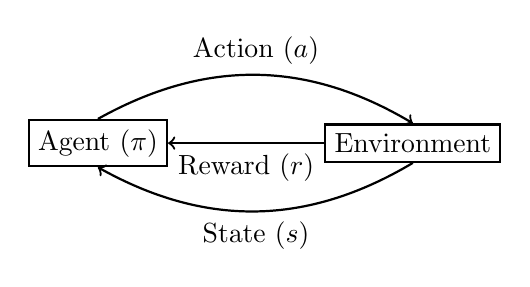
\begin{tikzpicture}[->, thick]
         %nodes
         \node[draw] at (-2,0) (agent) {Agent ($\pi$)}; % : S \to \mathcal{P}(A)
         \node[draw] at (2,0) (env) {Environment};
         \path
             (agent.north) edge[bend left=30] node[above] {Action ($a$)} (env.north)
             (env.south) edge[bend left=30] node[below] {State ($s$)} (agent.south)
             (env.west) edge node[below] {Reward ($r$)} (agent.east);
    \end{tikzpicture}
    % }
    \caption{The general reinforcement learning paradigm.}
    \label{fig:RL}
\end{figure}

The agent decides what actions to perform via a policy function $\pi$, which maps from a state $s \in S$ to either a probability distribution over the action space $\mathcal{P}(A)$ (a ``stochastic policy'') or simply a particular action $a \in A$ (a ``deterministic policy''). Policy functions are typically implemented as neural networks which are then usually optimized using gradient-based methods.

There are a few other common functions used in RL. The \emph{return} at time step $t$ is defined as
\begin{equation}\label{eq:return}
    G_t \defeq \sum_{k=t}^T \gamma^{k-t} R_k, \quad \gamma \in [0,1)
\end{equation}
or the total discounted rewards until the end of the episode at time step $T$. The \emph{state-value function} is the expected return from a particular state while following a policy $\pi$
\begin{equation}\label{eq:state_value}
    v_\pi(s) \defeq \E[G_t | S_t = s]
\end{equation}
Finally, the \emph{action-value function} is the expected return from taking an action $a$ in state $s$, then after following policy $\pi$
\begin{equation}\label{eq:action_value}
    q_\pi(s, a) \defeq \E[G_t | S_t = s, A_t = a]
\end{equation}

\subsection{Action space}

The action space can generally be discrete (there are finitely many actions that can be performed) or continuous  (infinitely many actions). The size of the action space determines the type of RL algorithm that can be used. In discrete action spaces, the policy can be stochastic and learn a probability distribution over every action. In continuous action spaces, where it's impractical to learn an arbitrary probability distribution over all actions, the policy can either be stochastic and learn parameters of a general probability distribution (such as a multivariate Gaussian) or deterministic and return the action.

For Hamiltonian engineering, the size of the action space depends on the number of allowed control Hamiltonians. As an example, in many pulse sequences developed using average Hamiltonian theory, the control Hamiltonians are restricted to $\pi/2$-pulses at consistent time intervals, which is better suited to a discrete action space. In contrast, techniques such as GRAPE
\cite{Khaneja-2005}
allow the control Hamiltonian amplitudes to vary continuously.

Both discrete and continuous action spaces were tested, and the results of each are shared below in the sections for each corresponding RL algorithm.

\subsection{Reward schemes}

The goal of Hamiltonian engineering is to control the system so that its time-evolution appears to be under some effective Hamiltonian. The reward signal should then be larger when the actual evolution is ``close'' to the target evolution. One measure of ``closeness'' is the fidelity function for two unitary operators
\begin{equation} % TODO make sure this is right
    F(U_\text{actual}, U_\text{target}) = \left| \frac{\Tr{
        U_\text{actual}^\dagger U_\text{target}
    }}{\Tr{\identity}} \right|
\end{equation}
The fidelity approaches 1 as the unitaries get closer, and approaches 0 as the unitaries get further apart. However, a tenfold improvement in performance doesn't correspond to a tenfold increase in fidelity (take for instance a fidelity of 0.9 compared to 0.99). A suitable reward function is then calculated by
\begin{equation}
    R = -\log(1-F(U_\text{actual}, U_\text{target}) + \epsilon)
\end{equation}
where $\epsilon>0$ ensures the reward isn't infinite.

There is also the decision of \emph{when} to give rewards to the agent. A reward can be given at every time step during the episode (``dense rewards'') or only at certain time steps such as the end of the episode (``sparse rewards'').
Dense rewards make sense when the fidelity matters at every time step, such as implementing a target unitary in the shortest amount of time possible.
% TODO does ^ make sense? May need to explain more...
Sparse rewards make sense when the fidelity only matters at certain points in time, such as in stroboscopic measurements and pulse sequences.

\subsection{State space and state representation}

The state space is the set of all possible states of the system. A possible approach would be to encode the state as the density matrix or propagator at the current time step. However, the density matrix and propagator grow exponentially as the system size increases, and the complete characterization of the quantum system is unrealistic for any experimental application.

An alternative state representation is the sequence of past actions applied to the system.  This representation generally requires less memory and computation, and may also be better suited to more robust control.

\subsection{Reinforcement Learning Taxonomy}

% TODO put in a diagram showing model-free, model, online, offline, etc....

\subsection{Algorithm Examples}

% TODO describe AlphaZero algorithm, others I tried?

There are many RL algorithms that have been developed, tailored to the specific characteristics of the problem. The relevant characteristics include
\begin{description}
    \item[Model] An agent in a \emph{model-free} RL algorithm learns a policy directly from observations of the environment. An agent in a \emph{model-based} RL algorithm instead uses observations to model the environment, then uses that model to learn a policy.
    \item[Policy] An \emph{on-policy} algorithm improves the policy that is used to interact with the environment. An \emph{off-policy} algorithm has separate policies for improvement and environment interaction.
    \item[Action space] As mentioned before, an action space can be \emph{discrete} (finitely many actions) or \emph{continuous} (infinitely many actions).
\end{description}
In addition to the above characteristics, there are general classes of RL algorithms, such as temporal-difference learning policy gradient methods. More information on RL can be found in \cite{sutton2018reinforcement}.

\subsubsection{Q-learning and DQN}

Q-learning is a model-free, off-policy, TD control algorithm applicable to discrete action spaces \cite{watkins1989learning}. As the name suggests, the action-value function $Q(s,a)$ is learned from experiences with the environment according to the following update rule
\begin{equation}\label{eq:Q_learning_update}
    Q(S_t, A_t) \leftarrow Q(S_t, A_t) +
        \alpha \left[ R_{t+1} + \gamma \max_a Q(S_{t+1}, a) - Q(S_t, A_t) \right]
\end{equation}
To encourage exploration of the state and action spaces, the agent typically follows an $\epsilon$-greedy policy (with probability $1-\epsilon$ perform the action that maximizes $Q$, otherwise perform a random action), which makes this algorithm \emph{off-policy}.

If the state and action spaces are small, then it's feasible for all the $Q$-values to be stored in memory. In general, though, the action-value function is approximated using a neural network, and the parameters are updated to minimize the loss given by \ref{eq:Q_learning_update}. This approach is called ``deep Q-network'' or DQN \cite{mnih2013playing}. DQN is suitable for large state spaces (as demonstrated through Atari games in \cite{mnih2013playing}), but still requires the action space to be discrete.

\subsubsection{DDPG}

``Deep deterministic policy gradient'' (DDPG) extends the idea of deep reinforcement learning in DQNs to continuous action spaces \cite{lillicrap2015continuous}. As with DQN, DDPG is a model-free, off-policy algorithm, but uses an actor-critic framework that separates the policy and the value function estimators. In addition, the policy is deterministic, so it returns a single action instead of a distribution over actions. As the agent interacts with the environment, the experiences are recorded in a \emph{replay buffer} on which the actor and critic are trained. The critic is updated by minimizing the sampled value estimate errors,
% TODO include update equation?
% \begin{align}\label{eq:DDPG_critic_update}
%     L = \frac{1}{N} \sum_i (y_i - Q(S_i, A_i | \theta^Q))^2 \\
%     y_i = R_i + \gamma Q'(S_{i+1}, \mu'(S_{i+1}|\theta^{\mu'}) |\theta^{Q'})
% \end{align}
and the actor is updated using the sampled policy gradient%
% TODO include?
% \begin{equation}
%     \nabla_{\theta^\mu} J \approx \frac{1}{N} \sum_i
%     \nabla_a Q(s, a | theta^Q)|_{s=s_i, a=\mu(s_i)}
%     \nabla_{\theta^\mu} \mu(s|\theta^\mu)|_{s_i}
% \end{equation}
.

\subsubsection{PPO}

Proximal-policy optimization (PPO) is a model-free, on-policy actor-critic algorithm that tried to improve data efficiency and robustness compared to existing algorithms (such as DQN or other policy gradient methods).
\cite{schulman2017proximal}.
In contrast with other policy gradient methods, the PPO objective function is clipped according to a hyperparameter $\epsilon$.
\begin{equation}\label{eq:ppo_loss}
    % eq 7 in PPO paper
    L(\theta) = \E_t \left[\min(
        r_t(\theta)\hat{A}_t,
        \text{clip}(r_t(\theta), 1-\epsilon, 1+\epsilon) \hat{A}_t
    )\right]
\end{equation}
where
$r_t(\theta) = \frac{\pi_\theta(a_t|s_t)}{\pi_{\theta'}(a_t|s_t)}$ is the probability ratio of actions under the new and old policies, and $\hat{A}_t$ is an estimator of the \emph{advantage function} at time $t$. By clipping the objective, the gradient updates are non-zero only for a region close to the previous policy, thus preventing policy changes that are too large.
PPO has been applied successfully to both continuous and discrete action spaces%
% TODO check above, I think that's right but not sure...
.

\subsubsection{ERL}

Evolutionary reinforcement learning (ERL) is a model-free, off-policy hybrid algorithm that uses both actor-critic policy gradient and evolutionary algorithm methods \cite{khadka2018evolutionguided}. ERL addresses problems found in many  gradient-based RL algorithms, including temporal credit assignment (associating actions to rewards that may be separated by many time steps), exploration of the state and action spaces, and policy convergence sensitivity to hyperparameters. To do so, ERL maintains a population of actors with individual policies that interact with the environment. The population's experiences are recorded in a shared replay buffer, and a separate actor/critic pair learn from the replay buffer using policy gradient (such as DDPG or DQN). Periodically, the policy gradient-based actor is copied into the population, and evolutionary algorithms are used to iterate a new ``generation'' of actors (by preferentially selecting high-performing actors). By using both gradient-based and gradient-free methods, ERL attempts to achieve both efficiency and policy diversity, making it a candidate for a variety of RL problems.

